% -*- TeX-master: "main" -*-

\section{Package syntax and semantics}
\label{sec:syntax}

This section contains a definition of the syntax and semantics of the Groups package for \sbmlthreecore.  The Groups package involves six new object classes, \Group, \Member, \MemberConstraints, \AttributeConstraint, \ListOfMembers and \ListOfGroups, as well as a simple extension of the existing \Model object class.  \sec{examples} contains complete examples of using the constructs in SBML models.

% --------------------------------------------------------------------------
\subsection{Namespace URI and other declarations necessary for using this package}
\label{xml-namespace}

Every SBML Level~3 package is identified uniquely by an XML namespace URI.  For an SBML document to be able to use a given Level~3 package, it must declare the use of that package by referencing its URI.  The following is the namespace URI for this version of the Groups package for \sbmlthreecore:
\begin{center}
\uri{http://www.sbml.org/sbml/level3/version1/groups/version1}
\end{center}

In addition, SBML documents using a given package must indicate whether understanding the package is required for complete mathematical interpretation of a model.  This is done using the attribute \token{required} on the \token{<sbml>} element in the SBML document.  For the Groups package, the value of this attribute must be \val{false}, because the use of the Groups package cannot change the mathematical meaning of a model.

The following fragment illustrates the beginning of a typical SBML model using \sbmlthreecore and this version of the Groups package:

\begin{example}
<?xml version="1.0" encoding="UTF-8"?>
<sbml xmlns="http://www.sbml.org/sbml/level3/version1/core" level="3" version="1"
      xmlns:groups="http://www.sbml.org/sbml/level3/version1/groups/version1"
      groups:required="false">
\end{example}


\subsection{Primitive data types}
\label{new-primitive-types}

The Groups package uses a number of the primitive data types described in Section~3.1 of the \sbmlthreecore specification, and adds one additional primitive type described below.


\subsubsection{Type \fixttspace\primtypeNC{GroupKind}}
\label{primtype-groupkind}

The \primtype{GroupKind} primitive data type is used in the definition of the \Group class.  \primtype{GroupKind} is derived from type \primtype{string} and its values are restricted to being one of the following possibilities: \val{classification}, \val{partonomy}, and \val{collection}.  Attributes of type \primtype{GroupKind} cannot take on any other values.  The meaning of these three values is discussed in the context of the \Group class' definition in \sec{group-class}.


\subsection{The \class{Group} class}
\label{group-class}

The first and most central class in the Groups package is the \Group class.  \fig{group-uml} provides the UML diagram of its definition.  The \Group class provides an optional identifier and name, one required attribute (\token{kind}), and two children:  a list of members of the group, and a \MemberConstraints child which imposes additional restrictions on those members.  These are described below.

Since \Group is derived from \SBase, and \SBase provides the ability to attach SBO terms as well as MIRIAM annotations, the semantics of a given group in a model can be made more precise by reference to external controlled vocabularies and ontologies.  This capability is discussed further in \sec{semantics}.


\subsubsection{The \fixttspace\tokenNC{id} and \fixttspace\tokenNC{name} attributes}
\label{group-idname-attributes}

The optional \token{id} attribute on the \Group object class serves to provide a way to identify a group.  The attribute takes a value of type \primtype{SId}.  Note that the identifier of a group carries no mathematical interpretation and cannot be used in mathematical formulas in a model.  \Group also has an optional \token{name} attribute, of type \primtype{string}.  The \token{name} attribute may be used in the same manner as other \token{name} attributes on \sbmlthreecore objects; please see Section~3.3.2 of the \sbmlthreecore specification for more information.


\begin{figure}[bh]
  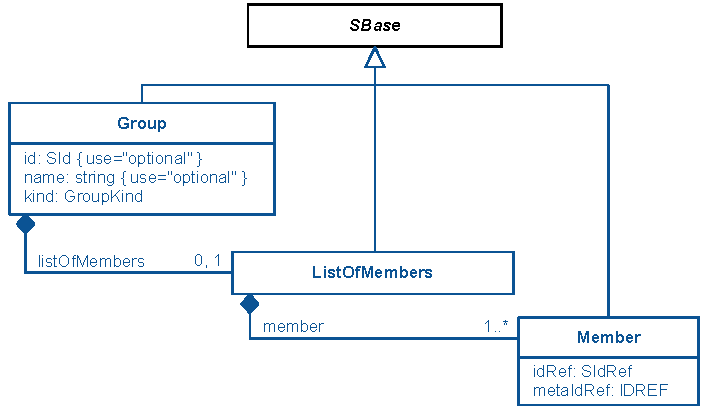
\includegraphics{figs/group-uml}
  \caption{The definition of the \Group class.  The \ListOfMembers, \Member, \MemberConstraints, and \AttributeConstraint classes are defined below.}
  \label{group-uml}
  \label{member-uml}
\end{figure}

\subsubsection{The \fixttspace\tokenNC{kind} attribute}
\label{kind-attribute}

\Group has one required attribute, \token{kind}, of type \primtype{GroupKind}.  This attribute is used to indicate the nature of the group defined by a \Group instance.  The \token{kind} attribute must always have one of the three possible values of \primtype{GroupKind}; these values have the following meanings:

\begin{description}[font=\normalfont\ttfamily\color{black},style=nextline]

\item[\token{classification}] The group represents a class, and its members have an \emph{is-a} relationship to the group.  (For example, the group could represent a type of molecule such as ATP, and the members could be species located in different compartments, thereby establishing that the species are pools of the same molecule in different locations.)

\item[\token{partonomy}] The group represents a collection of parts, and its members have a \emph{part-of} relationship to the group.  (For example, the group could represent a cellular structure, and individual compartments could be made members of the group to indicate they represent subparts of that cellular structure.)

\item[\token{collection}] The grouping is merely a collection for convenience, without an implied relationship between the members.  (For example, the group could be used to collect together multiple disparate components of a model---species, reactions, events---involved in a particular phenotype, and apply a common annotation rather than having to copy the same annotation to each component individually.)

\end{description}

\subsection{The \class{ListOfMembers} class}
\label{listofmembers-class}

The \ListOfMembers class is defined in \fig{member-uml}, and must have one or more \Member children.  Since \ListOfMembers is derived from \SBase, it inherits the \token{sboTerm} and \token{metaid} attributes, as well as the optional children \Notes and \Annotation.  Unlike most lists of objects in SBML, however, the \token{sboTerm} attribute and the \Notes and \Annotation children are taken here to apply directly to every SBML element referenced by each child \Member of this \ListOfMembers, if that referenced element has no such defintion.  If a referenced element has no defined \token{sboTerm}, that element should be considered to now have the \token{sboTerm} defined on the \ListOfMembers.  If a referenced element has no defined \Notes child, that element should be considered to now have the \Notes child of the \ListOfMembers.  If a referenced element has no defined \Annotation child, that element should be considered to now have the \Annotation child of the \ListOfMembers.

\emph{Note: \notice Alternatively, any annotations could be considered to additionally apply to the referenced member, as well as any annotation it may already have.}


\subsection{The \class{Member} class}
\label{member-class}

The \Member class is defined in \fig{member-uml}.  It has two optional attribute, \token{id} and \token{name} that allow others to reference it, and two optional attributes, \token{idRef} and \token{metaIdRef} that allow it to reference other elements, exactly \emph{one} (and only one) of which must have a value in a given \Member object instance.  The referenced object (including, potentially, another \Group object) is thus made a member of the group in which the \Member object is contained.  Multiple attributes are needed to account for the different types of identifiers that a given object may have.  The meaning and purpose of the attributes on the object class are described below.

Since \Member is derived from \SBase and, as mentioned above, \SBase provides both the ability to attach SBO terms as well as MIRIAM annotations, the semantics of a given member in a model can be made more precise by reference to external controlled vocabularies and ontologies.


\subsubsection{The \fixttspace\tokenNC{id} and \fixttspace\tokenNC{name} attributes}
\label{member-idname-attributes}

The optional \token{id} attribute on the \Member object class serves to provide a way to identify the member reference.  The attribute takes a value of type \primtype{SId}.  Note that the identifier of a member reference carries no mathematical interpretation and cannot be used in mathematical formulas in a model.  \Member also has an optional \token{name} attribute, of type \primtype{string}.  The \token{name} attribute may be used in the same manner as other \token{name} attributes on \sbmlthreecore objects; please see Section~3.3.2 of the \sbmlthreecore specification for more information.


\subsubsection{The \fixttspace\tokenNC{idRef} attribute}
\label{member-idref-attribute}

The attribute \token{idRef} on the \Member class has type \primtype{SIdRef}, and must be defined if the \Member has no defined \token{metaIdRef} attribute, and must not be defined otherwise.  The value must be the identifier of an object elsewhere in the \Model.  (Object identifiers are usually set by attributes named \token{id}; thus, the \token{idRef} value will usually be the \token{id} value of an object in the \Model.)  An example value of \token{idRef} might be the identifier of a species in the model, or the identifier of another group.  The namespace in which the \primtype{SId} is to be found is the SId namespace of the \Model to which the \Group belongs.  This includes elements from SBML packages which may have elements with \token{id} values that are part of the SId namespace of the \Model, such as \Deletion elements from the Hierarchical Model Composition package, \FluxBound elements from the Flux Balance Constraints package, and \Group, \Member, \MemberConstraints, and \AttributeConstraint elements from this Groups package.  Conversely, elements with \token{id} values that are not part of the SId namespace of the \Model such as \Unit and \LocalParameter elements in \sbmlthreecore, or \Port elements from the Hierarchical Model Composition package, may not be referenced by this \token{idRef} attribute.


\subsubsection{The \fixttspace\tokenNC{metaIdRef} attribute}
\label{member-metaidref-attribute}

The \Member attribute \token{metaIdRef} takes a value of type \primtype{IDREF}, and must be defined if the \Member has no defined \token{idRef} attribute, and must not be defined otherwise.  This attribute is used to refer to a \token{metaid} attribute value on some other object in the SBML Document, for cases where the object being referenced does not have an identifier in the \Model SId namespace, or is not a direct member of the same \Model.  (This is the case with, for example, rules in \sbmlthreecore.)  Since meta identifiers are optional attributes of \SBase, all SBML objects have the potential to have a meta identifier value, including most elements from other SBML packages.

Note that if used in conjunction with the Hierarchical Model Composition package, this attribute can reference elements from other \Model objects in the same SBML Document!  It is suggested, but not required, that if a \Member object is created with such a reference, that reference be part of one or more \Submodels of the \Model parent of this \Group.  Further, it is suggested that if the \Model is flattened, that a separate \Member be created for each instance of the referenced element present in the flattened \Model (which will happen if the referenced element's \Model is instantiated by multiple \Submodel elements).

\subsubsection{Members referencing other Groups and Members}
\label{recursive-groups}

If a \Member references a \Group or \ListOfMembers element, all the members of the referenced group are considered to be part of the parent group--this is equivalent to adding the members of the referenced group individually as members.  This means that any semantic restrictions or imlications of adding elements to this group apply to the referenced elements, and \emph{not} to the reference itself.  In other words, if a \ListOfMembers is annotated with an SBO term, and the \token{idRef} of a \Member child points to a different \Group, it is not that \Group that should be annotated with the SBO term, but its referenced members.  This applies recursively:  if the referenced \Group itself has referenced \Group members, those reference should also be discovered and annotated with the SBO term.

A \Member referencing another \Member object is considered equivalent to pointing at the referenced element directly.  This is discouraged, and modelers are encouraged to point to the referenced element directly instead.

\subsubsection{Members referencing other namespaces}
\label{unfindable-members}

If a \Member has a \token{idRef} or \token{metaIdRef} attribute which references an object from a namespace that is not understood by the interpreter, that \Member must be ignored---the object will not exist to need to become a member of the group, as the interpreter could not understand the package. If an interpreter cannot tell whether a referenced object does not exist or if exists in an unparsed namespace, it may choose to produce a warning.




\subsubsection{Example}

As mentioned above, exactly one of the attributes \token{idRef} and \token{metaIdRef} must have a value in a given \Member object instance.  There are no restrictions on mixing the attributes used across multiple members of the same group, however.  The following artificial example illustrates the definition of a heterogeneous group, as well as the use of nested groups:

\begin{example}
...
  <listOfSpecies>     
      <species id="S1" compartment="c" initialConcentration="1"/> 
      <species id="S2" compartment="c" initialConcentration="2"/> 
  </listOfSpecies>   
  <listOfCompartments>   
      <compartment id="C" size="1"/>
  </listOfCopartments>   
  <listOfRules>
      <rateRule variable="S2" metaid="_rule1">
          <math xmlns="http://www.w3.org/1998/Math/MathML">
              <apply>
                  <times/>
                  <ci> S1 </ci>
                  <cn> 0.5 </cn>
              </apply>
          </math>
      </rateRule>
  </listOfRules>
  <listOfGroups xmlns="http://www.sbml.org/sbml/level3/version1/groups/version1">   
      <group id="all_species" kind="collection">
          <listOfMembers>
              <member idRef="S1"/> 
              <member idRef="S2"/> 
          </listOfMembers>
      </group> 
      <group id="all_entities" kind="collection">
          <listOfMembers>
              <member idRef="all_species"/> 
              <member idRef="C"/> 
              <member metaIdRef="_rule1"/> 
          </listOfMembers>
      </group> 
  </listOfGroups>   
...
\end{example}


\subsection{The \class{MemberConstraints} class}
\label{memberconstraints-class}

The \MemberConstraints class is defined in \fig{group-uml} as a way to impose restrictions on the referenced member elements of a \Group.  It can be used to ensure that all members of a group are of the same SBML Class; that all members of a group have the same parent, or to ensure that all members of the group have the same attribute with the same value or with all different values.

It has one required attribute, \token{membersShareType}, and three optional attributes: \token{idRef} and \token{metaIdRef}, and \token{membersShareParent}.  It also may contain one or more \AttributeConstraint child objects, all described below.

\subsubsection{The \fixttspace\tokenNC{id} and \fixttspace\tokenNC{name} attributes}
\label{memberconstraints-idname-attributes}

The optional \token{id} attribute on the \MemberConstraints object class serves to provide a way to identify the constraints.  The attribute takes a value of type \primtype{SId}.  Note that this identifier carries no mathematical interpretation and cannot be used in mathematical formulas in a model.  \MemberConstraints also has an optional \token{name} attribute, of type \primtype{string}.  The \token{name} attribute may be used in the same manner as other \token{name} attributes on \sbmlthreecore objects; please see Section~3.3.2 of the \sbmlthreecore specification for more information.


\subsubsection{The \fixttspace\tokenNC{membersShareType} attribute}
\label{memberssharetype-attribute}

The required attribute \token{membersShareType} on the \MemberConstraints class has type \primtype{boolean}.  If set to \val{true}, all referenced members of the \Group must be the same exact SBML class.  This means that sharing a base class (such as \SBase or \Rule) is insufficient: an \AlgebraicRule and a \RateRule are different classes from one another.

If set to \val{false}, the referenced members of the \Group may be of any SBML class; no restrictions are implied.


\subsubsection{The \fixttspace\tokenNC{membersShareParent} attribute}
\label{membersshareparent-attribute}

The optional attribute \token{membersShareParent} on the \MemberConstraints class has type \primtype{IDREF}.  If set, it must reference the \token{metaid} of an element of the SBML Document.  Furthermore, all referenced members of the \Group must share that element as a common parent, either directly or indirectly.  As an example, a \KineticLaw and a \LocalParameter might share the same \Reaction parent, even though the immediate parent of the \LocalParameter is a \ListOfLocalParameters.

If unset, no implication is made about the common parent of the referenced members of the \Group.

If a \token{membersShareParent} attribute references an object from a namespace that is not understood by the interpreter, the restriction of shared parentage can be ignored, though the interpreter may conclude that if it can properly reference one or more group members, it would have to be able to understand the parents of those members.  If an interpreter cannot tell whether a referenced object does not exist or if exists in an unparsed namespace, it may choose to produce a warning.



\subsection{The \class{AttributeConstraint} class}
\label{attributeconstraint-class}

The \AttributeConstraint class is defined in \fig{group-uml} as a way to impose restrictions on common attributes of the referenced members of the \Group.  It has two optional attributes to identify the attribute constraint itself (\token{id} and \token{name}), and two other optional attributes (\token{identicalAttribute} and \token{distinctAttribute}) of which exactly \emph{one} (and only one) must be defined.

\subsubsection{The \fixttspace\tokenNC{id} and \fixttspace\tokenNC{name} attributes}
\label{attributeconstraint-idname-attributes}

The optional \token{id} attribute on the \AttributeConstraint object class serves to provide a way to identify the \AttributeConstraint.  The attribute takes a value of type \primtype{SId}.  Note that this identifier carries no mathematical interpretation and cannot be used in mathematical formulas in a model.  \AttributeConstraint also has an optional \token{name} attribute, of type \primtype{string}.  The \token{name} attribute may be used in the same manner as other \token{name} attributes on \sbmlthreecore objects; please see Section~3.3.2 of the \sbmlthreecore specification for more information.


\subsubsection{The \fixttspace\tokenNC{distinctAttribute} attribute}
\label{distinctattribute-attribute}

The attribute \token{distinctAttribute} on the \AttributeConstraint class has type \primtype{string}.  This attribute must be defined if the \AttributeConstraint has no defined \token{identicalAttribute}, and must not be defined otherwise.  The value of the string must be the name of an attribute shared by all referenced members of the \Group.  Furthermore, the \emph{values} of those attribute must be different across all referenced elements.  The rule from SBML Level~2 that no two \SpeciesType elements may share a compartment could be enforced here by setting this attribute to \val{compartment}.


\subsubsection{The \fixttspace\tokenNC{identicalAttribute} attribute}
\label{identicalattribute-attribute}

The attribute \token{identicalAttribute} on the \AttributeConstraint class has type \primtype{string}.  This attribute must be defined if the \AttributeConstraint has no defined \token{distinctAttribute}, and must not be defined otherwise.  The value of the string must be the name of an attribute shared by all referenced members of the \Group.  Furthermore, the \emph{values} of those attributes must be the same for all referenced elements.  If the referenced members are all \Species, for example, this attribute might be set to be \val{boundaryCondition}, ensuring that all the referenced elements have the same value (\val{true} or \val{false}).  If these species all represented the concentration of dissolved oxygen in various different compartments, another \AttributeConstraint could be set with an \token{identicalAttribute} of \val{initialConcentration}, ensuring that the initial concentration of dissolved oxygen was the same across all compartments.

\subsubsection{Example}

A partial example of a working \MemberConstraints element is shown below.  In it, the two referenced members (\val{ATPc} and \val{ATPm}) are declared to be the same type using the \token{membersShareType} attribute, that they must have different compartments with a \token{distinctAttribute} attribute, and that they must both have the same initial concentration with a \token{identicalAttribute} attribute. 

\begin{example}
    <group id="ATP" kind="classification"> 
        <listOfMembers sboTerm="SBO:0000248">
            <member idRef="ATPc" />
            <member idRef="ATPm" />
        </listOfMembers>
        <memberConstraints membersShareType="true">
            <attributeConstraint distinctAttribute="compartment" />
            <attributeConstraint identicalAttribute="initialConcentration" />
        </memberConstraints>
    </group> 
\end{example}

A complete SBML document including the above snippet is included in \sec{examples-speciestype}.

\subsection{The extended \class{Model} class}
\label{model-class}
\label{extended-model-class}
\label{listofgroups-class}

The Groups package extends \sbmlthreecore's \Model class to add one list, \ListOfGroups, for holding group definitions.  \fig{extended-model-uml} provides the UML diagram for the extension.

\begin{figure}[hbt]
  \begin{overpic}{figs/group-model-uml}
    \put(85.25,12.75){\emph{\sec*{group-class}}}
  \end{overpic}
  \caption{The extensions of the \Model class.  \Group is defined in \sec{group-class}. In other respects, \Model remains defined as in the \sbmlthreecore specification.}
  \label{extended-model-uml}
\end{figure}


\subsubsection{The list of groups}

\fig{extended-model-uml} shows that the extension of \Model by the Groups package involves adding optional \token{listOfGroups} subcomponent for holding a \ListOfGroups container object.  If present, the \ListOfGroups instance must contain at least one \Group object (\sec{group-class}).  In common with other \textsf{\textbf{ListOf\rule{0.15in}{0.5pt}}} classes in SBML, \ListOfGroups is derived from \SBase.  It inherits \SBase's attributes \token{metaid} and \token{sboTerm}, as well as the subcomponents for \Annotation and \Notes, but does not add any new attributes of its own.


\section{The semantics of ``groups''}
\label{semantics}

A group \emph{G} is defined by declaring an instance of a \Group class object within the \ListOfGroups element of a \Model object. The group can be given an optional identifier (i.e., a value for its \token{id} attribute), but even if the group does not have an identifier, the act of declaring a group has the effect of creating it.

An entity \emph{X} in the model is declared to be part of group \emph{G} by listing the identifier of \emph{X} in a \Member object within the \ListOfGroups instance of \emph{G}. The following is an example to illustrate the structure:

\begin{example}
<model id="model_1"> 
  <listOfSpecies> 
    <species id="s1" .../> 
    <species id="s2" .../> 
    <species id="s3" .../> 
    <species id="s4" .../> 
  </listOfSpecies> 
  ... 
  <listOfReactions> 
    <reaction id="r1" ...> ... </reaction> 
    <reaction id="r2" ...> ... </reaction> 
  <listOfReactions> 
  ... 
  <listOfGroups xmlns="http://www.sbml.org/sbml/level3/version1/groups/version1"> 
    <group id="some_species_group" kind="collection"> 
      <listOfMembers> 
        <member idRef="s1"/> 
        <member idRef="s3"/> 
      </listOfMembers> 
    </group> 
    <group id="some_reaction_group" kind="collection"> 
      <listOfMembers> 
        <member idRef="r1"/> 
        <member idRef="r2"/> 
      </listOfMembers> 
    </group> 
  </listOfGroups> 
</model>
\end{example}

For any given group, the meaning of group membership is determined by the value of the attribute \token{kind} on the \Group object instance.  Examples of possible meanings are given in \sec{kind-attribute}.

The meaning of a group can be further refined by using annotations (either SBO terms or the \Annotation element) on the group, or the list of members. The following are the interpretations.  This possibility raises the question of how the annotations should be interpreted across the group members.  The following are the possibilities defined by the Groups package:

\begin{itemize}

\item If the annotation or SBO term is on a \Group object, it is an annotation about the group itself, not the individual members.

\item If the annotation or SBO term is on a \Member object, it is an annotation specifically about that member, and not about any other member nor the group overall.

\item If the annotation or SBO term is on \ListOfMembers, it is a short-hand that means the annotation applies to each individual member, as if the annotation were put on the individual members directly.

\end{itemize}

Finally, as mentioned in \sec{member-class} above, groups can refer to other groups, leading to the possibility of group hierarchies. To indicate a group is part of another group, one simply needs to include the first group's identifier as a member of the second group, as in the following example:

\clearpage

\begin{example}
<model id="model_2"> 
  ... 
  <listOfGroups xmlns="http://www.sbml.org/sbml/level3/version1/groups/version1"> 
    <group id="group1"> 
      <listOfMembers> 
        <member idRef="..."/> 
        <member idRef="..."/> 
      </listOfMembers> 
    </group> 
    <group id="group2"> 
      <listOfMembers> 
        <member idRef="group1"/> 
        <member idRef="..."/> 
        <member idRef="..."/> 
      </listOfMembers> 
    </group> 
  </listOfGroups> 
</model> 
\end{example}

The intended meaning of nested groups can be made more precise by annotating the group and list of members with appropriate MIRIAM annotations using controlled vocabulary terms that describe the meaning.


\subsection{Semantic restrictions}
\label{semantic-restrictions}

The current definition of the Groups package is such that the use of Groups constructs has no impact on the mathematics of a model.  As a consequence of this, this package is not required for proper interpretation of a model. Models must use the \token{required}=\val{false} flag on the declaration of the package on the \token{<sbml>} element in a file.

Because restrictions can be imposed on the group through the use of the \MemberConstraints element, the Groups package can fully recapture SBML Level~2's \SpeciesType construct: a modeler can add an \AttributeConstraint to the group imposing the restriction that two \Species objects in the same \Group cannot have the same value for their respective \token{compartment} attributes.  A fully worked example (which also imposes additional restrictions) is given in \sec{examples-speciestype}.
